% Options for packages loaded elsewhere
\PassOptionsToPackage{unicode}{hyperref}
\PassOptionsToPackage{hyphens}{url}
\documentclass[
]{article}
\usepackage{xcolor}
\usepackage{amsmath,amssymb}
\setcounter{secnumdepth}{-\maxdimen} % remove section numbering
\usepackage{iftex}
\ifPDFTeX
  \usepackage[T1]{fontenc}
  \usepackage[utf8]{inputenc}
  \usepackage{textcomp} % provide euro and other symbols
\else % if luatex or xetex
  \usepackage{unicode-math} % this also loads fontspec
  \defaultfontfeatures{Scale=MatchLowercase}
  \defaultfontfeatures[\rmfamily]{Ligatures=TeX,Scale=1}
\fi
\usepackage{lmodern}
\ifPDFTeX\else
  % xetex/luatex font selection
\fi
% Use upquote if available, for straight quotes in verbatim environments
\IfFileExists{upquote.sty}{\usepackage{upquote}}{}
\IfFileExists{microtype.sty}{% use microtype if available
  \usepackage[]{microtype}
  \UseMicrotypeSet[protrusion]{basicmath} % disable protrusion for tt fonts
}{}
\makeatletter
\@ifundefined{KOMAClassName}{% if non-KOMA class
  \IfFileExists{parskip.sty}{%
    \usepackage{parskip}
  }{% else
    \setlength{\parindent}{0pt}
    \setlength{\parskip}{6pt plus 2pt minus 1pt}}
}{% if KOMA class
  \KOMAoptions{parskip=half}}
\makeatother
\usepackage{graphicx}
\makeatletter
\newsavebox\pandoc@box
\newcommand*\pandocbounded[1]{% scales image to fit in text height/width
  \sbox\pandoc@box{#1}%
  \Gscale@div\@tempa{\textheight}{\dimexpr\ht\pandoc@box+\dp\pandoc@box\relax}%
  \Gscale@div\@tempb{\linewidth}{\wd\pandoc@box}%
  \ifdim\@tempb\p@<\@tempa\p@\let\@tempa\@tempb\fi% select the smaller of both
  \ifdim\@tempa\p@<\p@\scalebox{\@tempa}{\usebox\pandoc@box}%
  \else\usebox{\pandoc@box}%
  \fi%
}
% Set default figure placement to htbp
\def\fps@figure{htbp}
\makeatother
\setlength{\emergencystretch}{3em} % prevent overfull lines
\providecommand{\tightlist}{%
  \setlength{\itemsep}{0pt}\setlength{\parskip}{0pt}}
\usepackage{bookmark}
\IfFileExists{xurl.sty}{\usepackage{xurl}}{} % add URL line breaks if available
\urlstyle{same}
% fallback for those not using the hyperref driver hyperxmp:
\makeatletter
\@ifundefined{xmpquote}{\newcommand{\xmpquote}[1]{#1}}{}
\makeatother
\hypersetup{
  hidelinks,
  pdfcreator={LaTeX via pandoc}}

\author{}
\date{}

\begin{document}

\section{3.5. Admin Management}\label{admin-management}

\subsection{3.5.1. User Management}\label{user-management}

Role: Amin

Function trigger: The admin opens the Admin page and selects Quản lý
người dùng.

Function description:

- Purpose: Allow the admin to manage user accounts in the system.

- Data processing: Retrieve user information from the database and
update user status or role.

Function Details:

- Display the list of users.

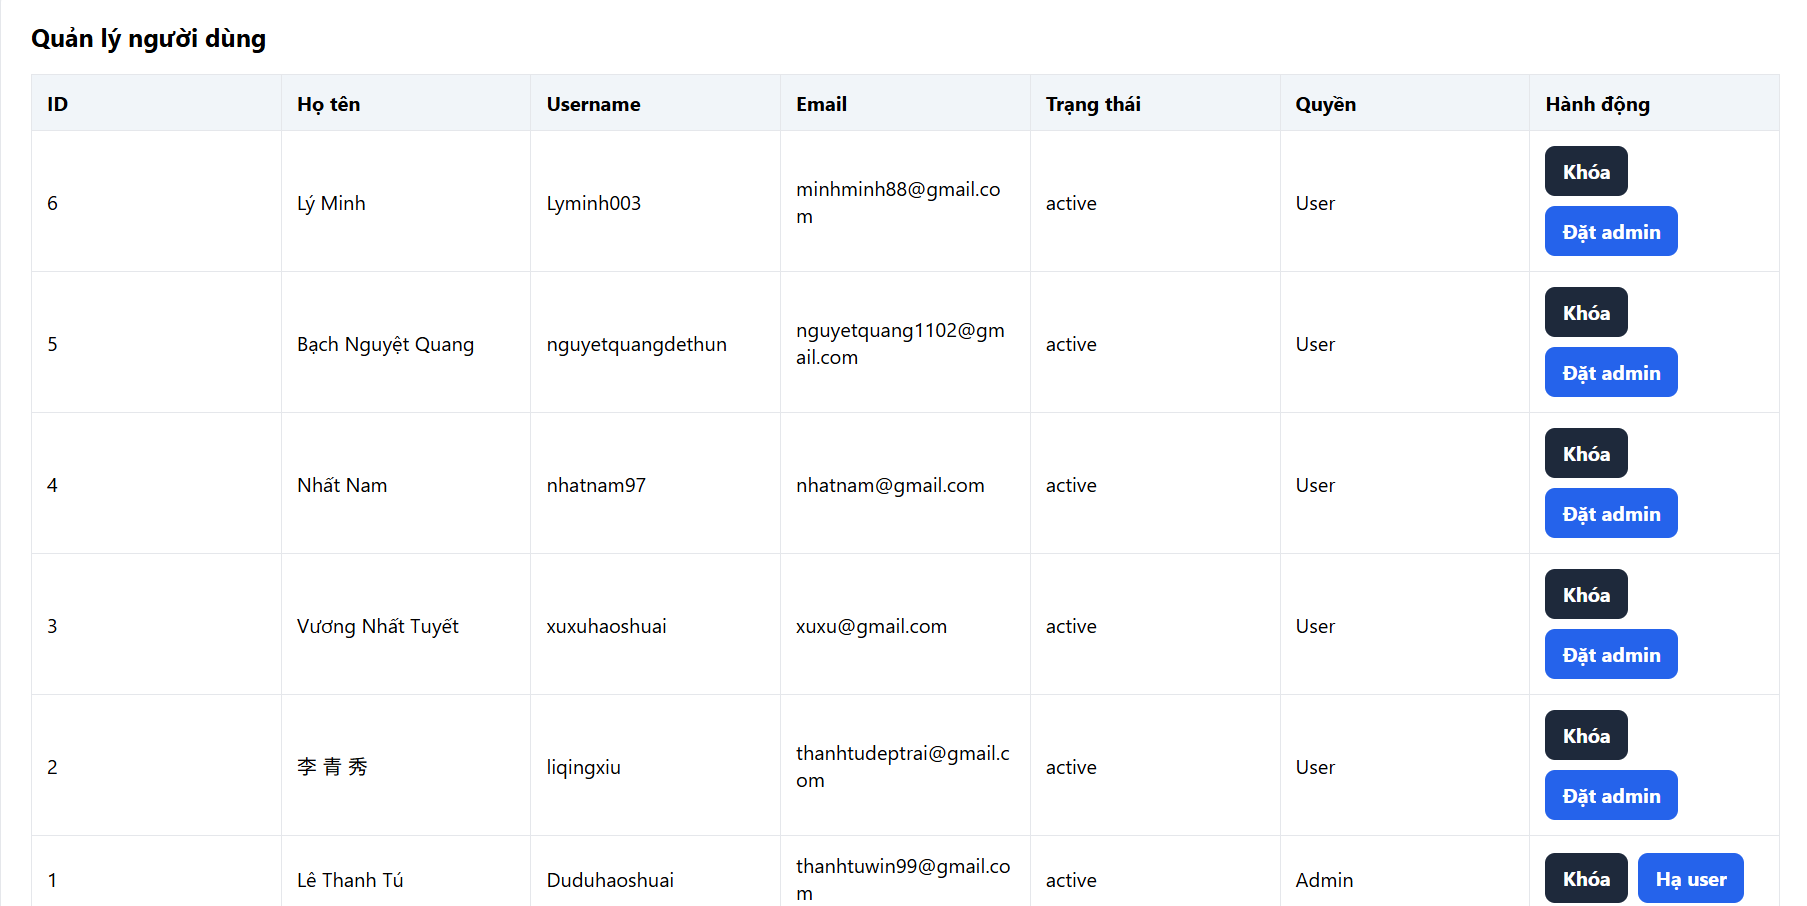
\includegraphics[width=6.5in,height=3.25903in]{media/media/image1.png}

\emph{Figure 3.1. Display the list of users.}

- Lock or unlock a user account.

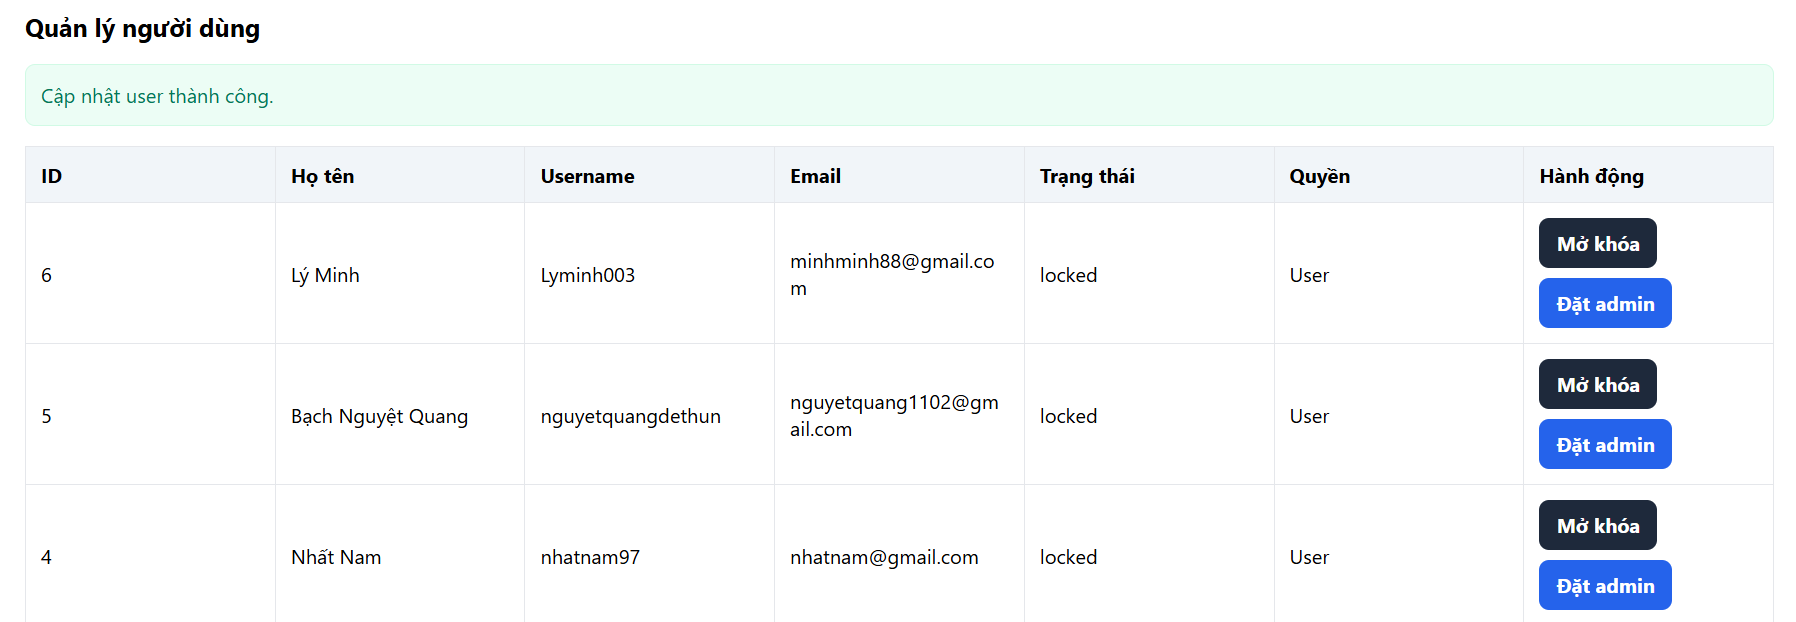
\includegraphics[width=6.5in,height=2.25069in]{media/media/image2.png}

\emph{Figure 3.2. Lock or unlock a user account}

- Assign admin role to a user.

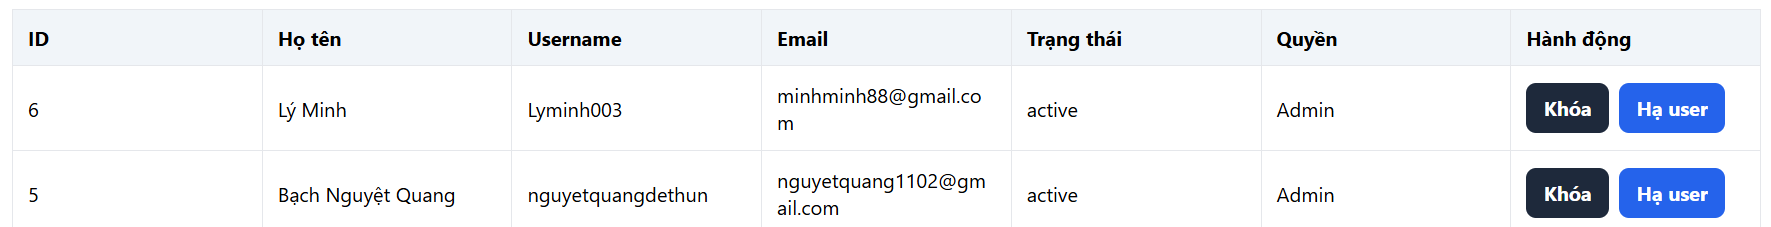
\includegraphics[width=6.5in,height=0.83333in]{media/media/image3.png}

\emph{Figure 3.3. Assign admin role to a user}

- Change an admin account back to a normal user.

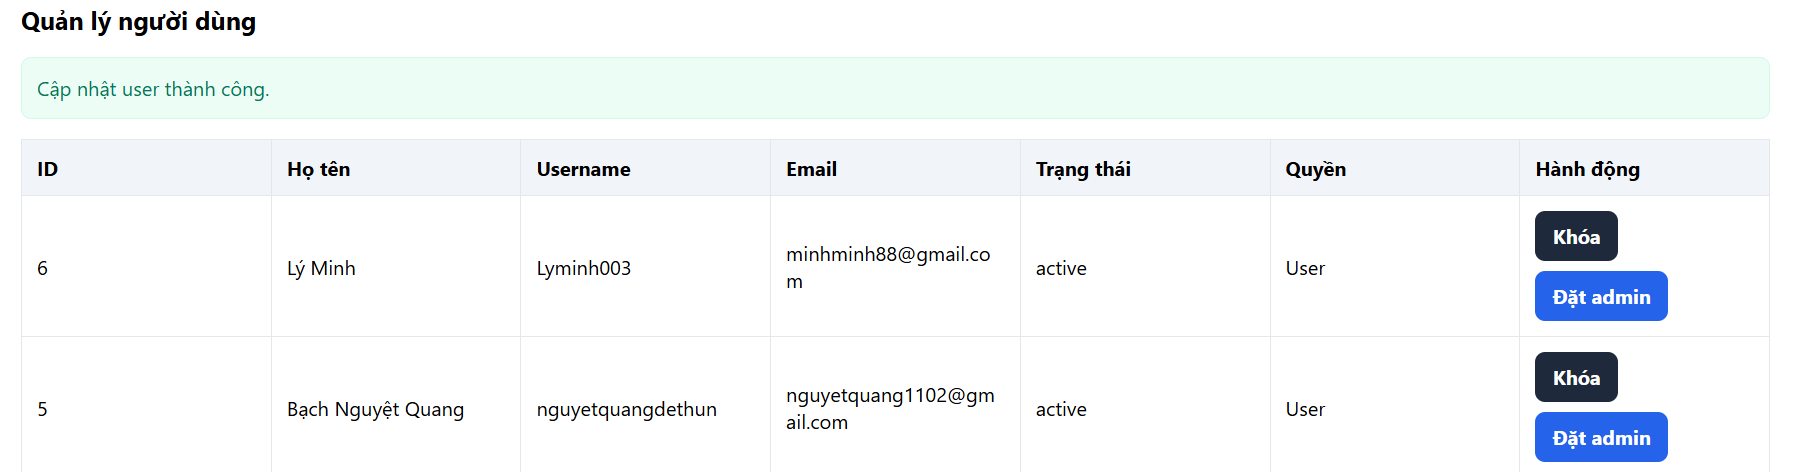
\includegraphics[width=6.5in,height=1.70694in]{media/media/image4.png}

\emph{Figure 3.4.Change an admin account back to a normal user }

- Display a success or error message after each action.

\subsection{3.5.2. Topic Management}\label{topic-management}

Role: Admin

Function trigger: The admin opens the Admin page and selects Quản lý chủ
đề.

Function description:

- Purpose: Allow the admin to manage research topics.

- Data processing: Add, update, delete, and retrieve topic data from the
database.

Function Details:

- Display the list of research topics.

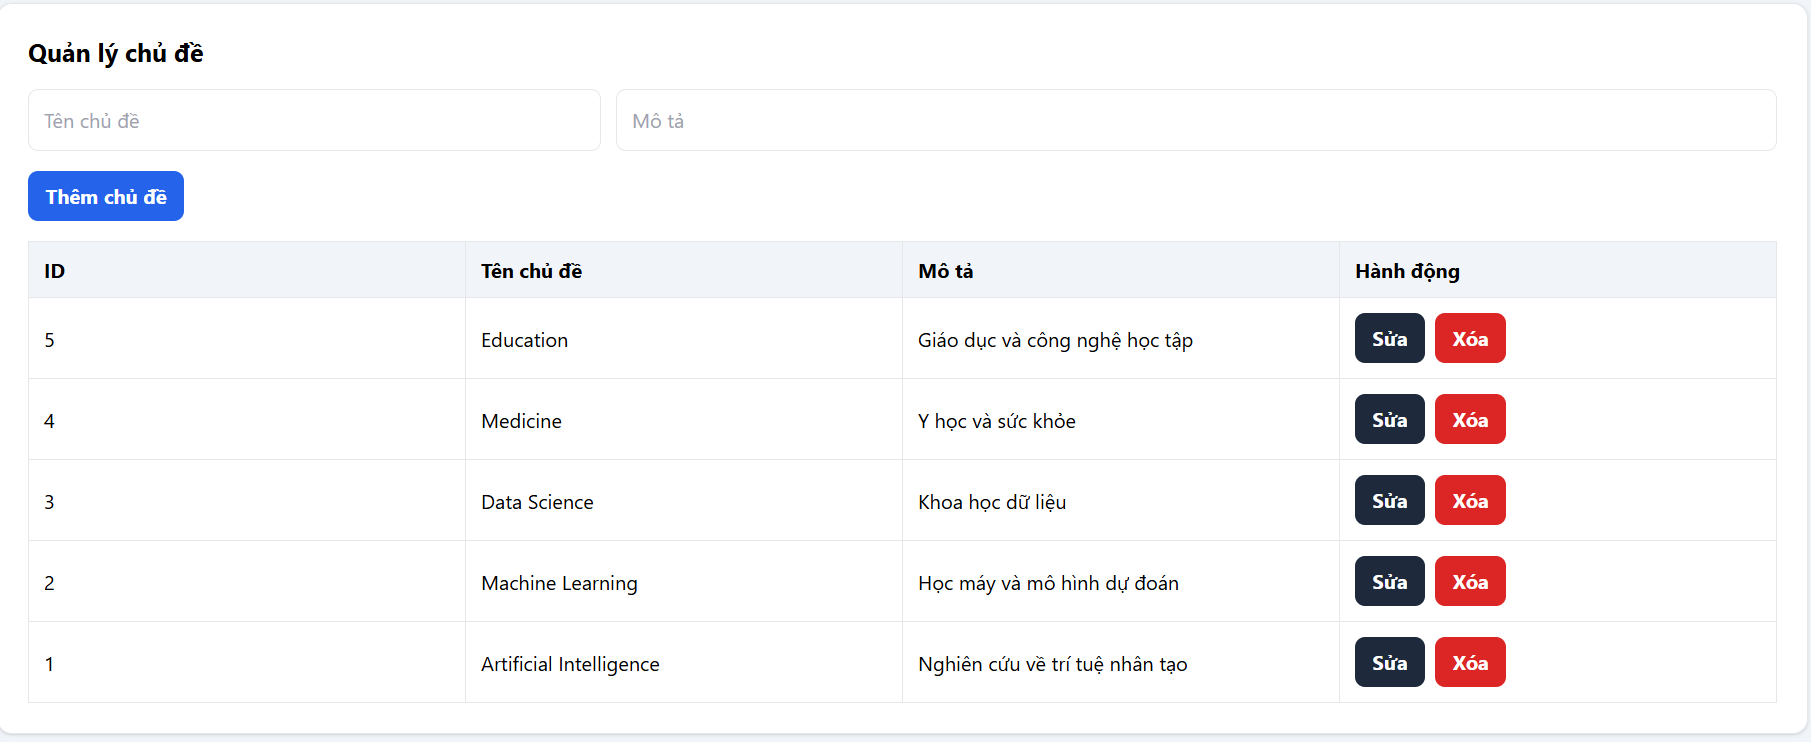
\includegraphics[width=6.5in,height=2.66319in]{media/media/image5.png}

\emph{Figure 3.5. Topic management interface displaying the list of
research topics.}

- Add a new topic with name and description.

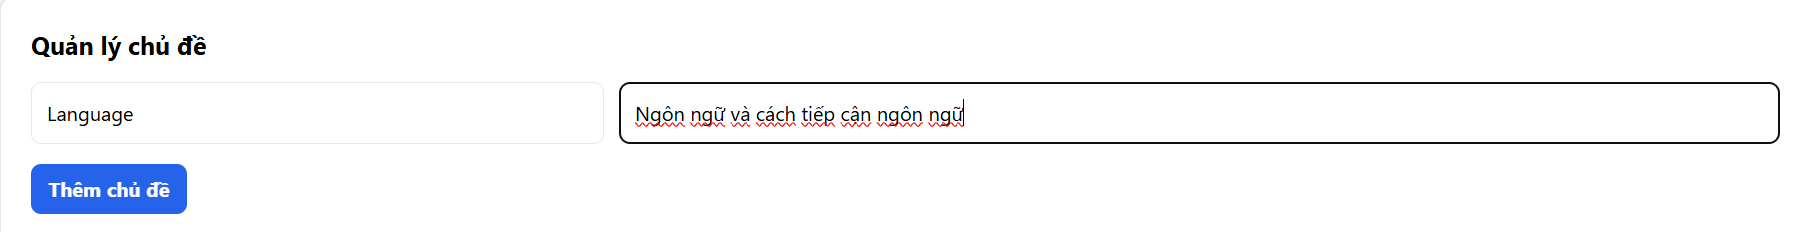
\includegraphics[width=6.5in,height=0.83681in]{media/media/image6.png}

\emph{Figure 3.6. Admin can add a new research topic by entering the
topic name and description.}

- Edit an existing topic.

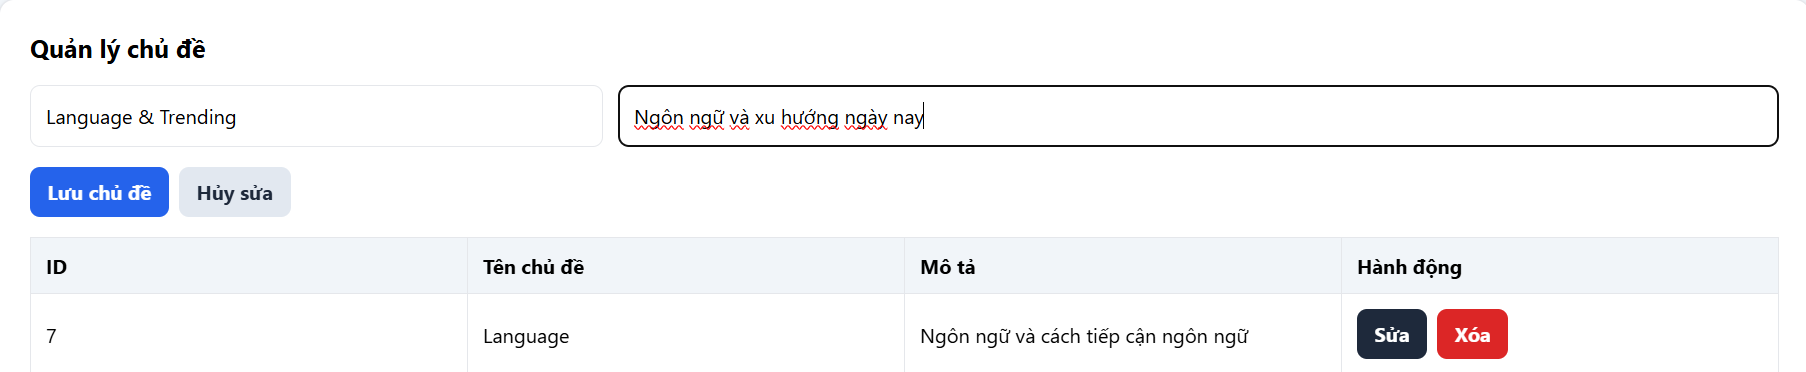
\includegraphics[width=6.5in,height=1.33889in]{media/media/image7.png}

\emph{Figure 3.7. Admin can edit an existing research topic.}

- Delete a topic.

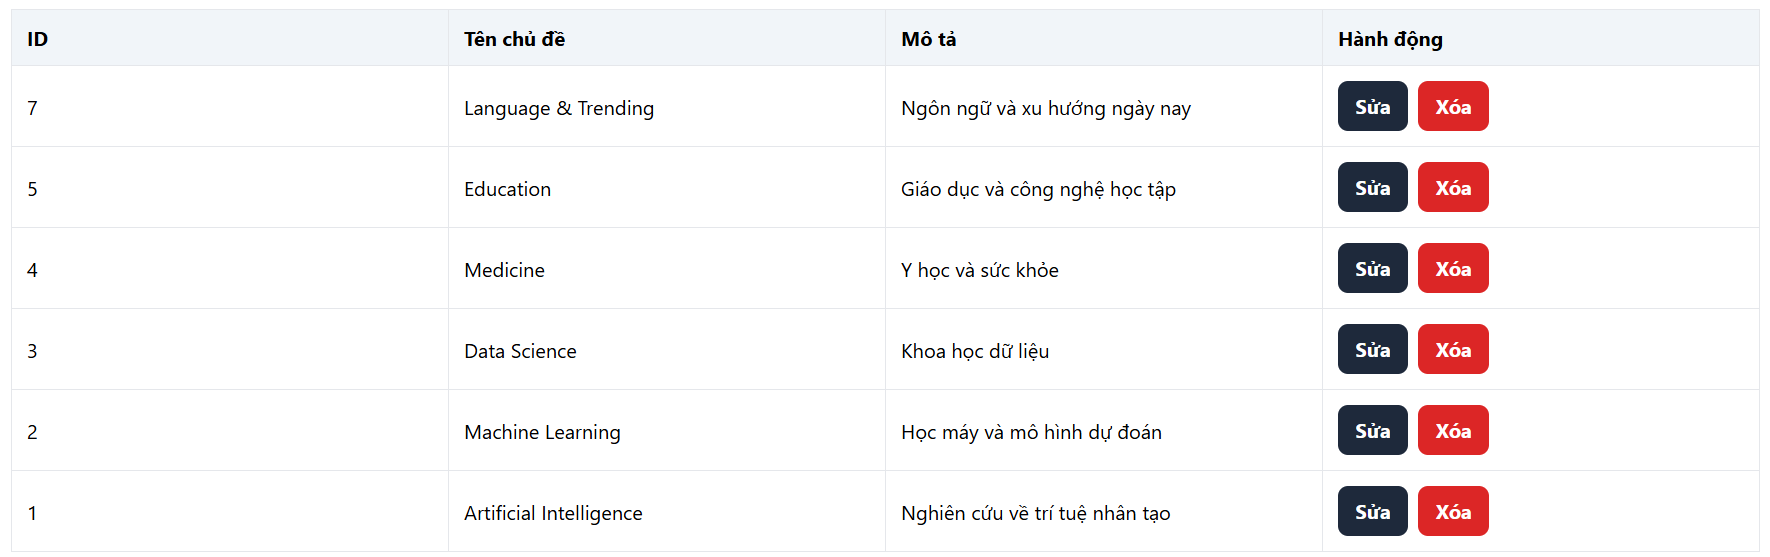
\includegraphics[width=6.5in,height=2.04514in]{media/media/image8.png}

\emph{Figure 3.8. Normal state}

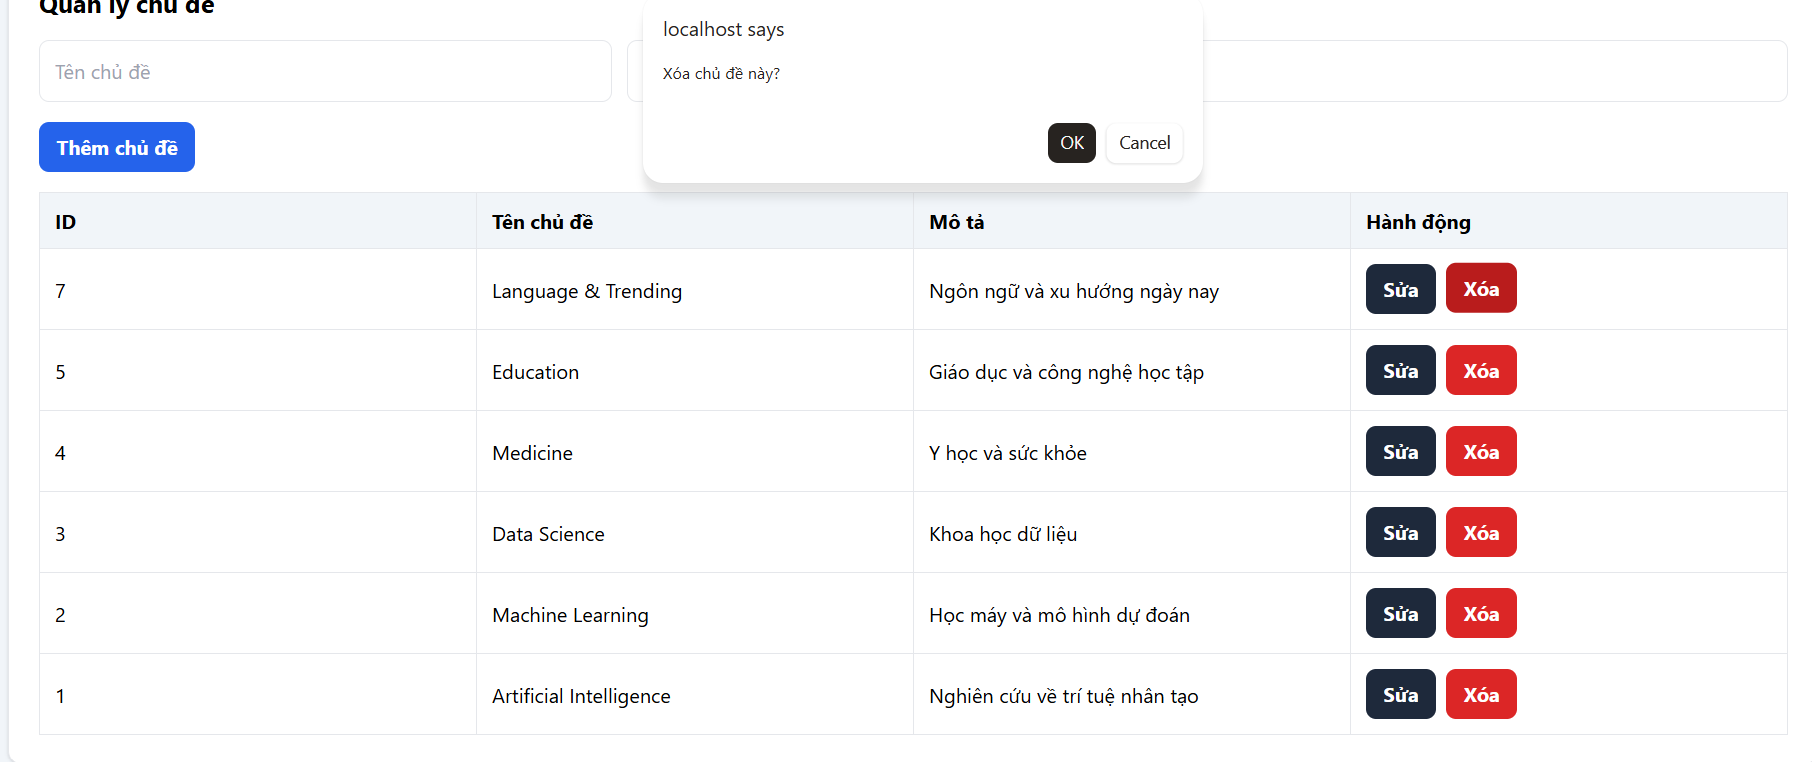
\includegraphics[width=6.5in,height=2.73333in]{media/media/image9.png}

\emph{Figure 3.9. Question ``Xóa chủ đề này?''}

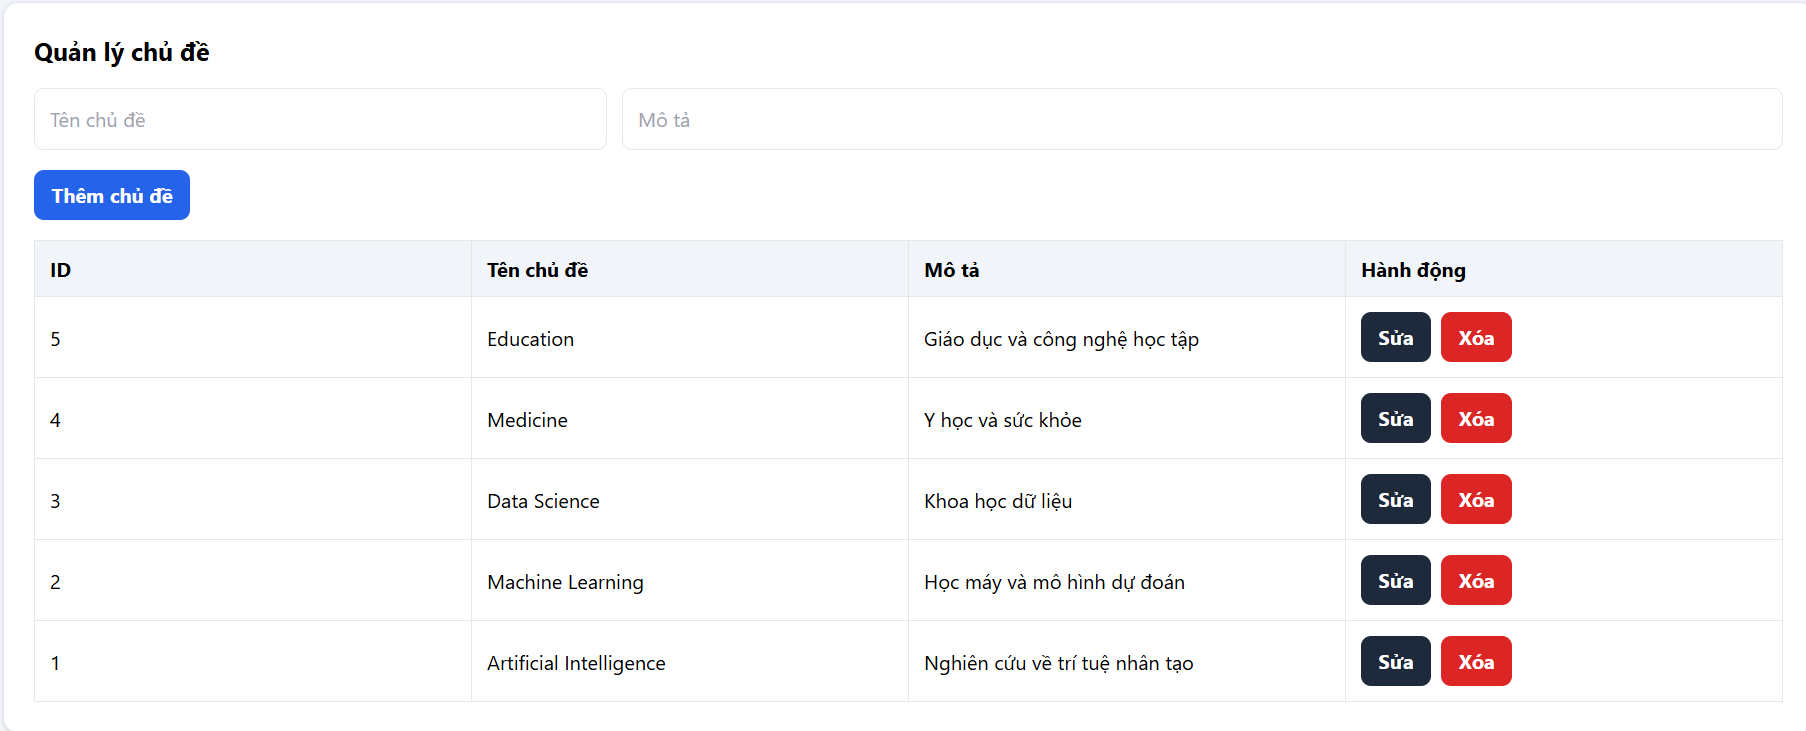
\includegraphics[width=6.5in,height=2.63056in]{media/media/image10.png}

\emph{Figure 3.10. Admin can delete an existing research topic.}

- Update the topic list after each action.

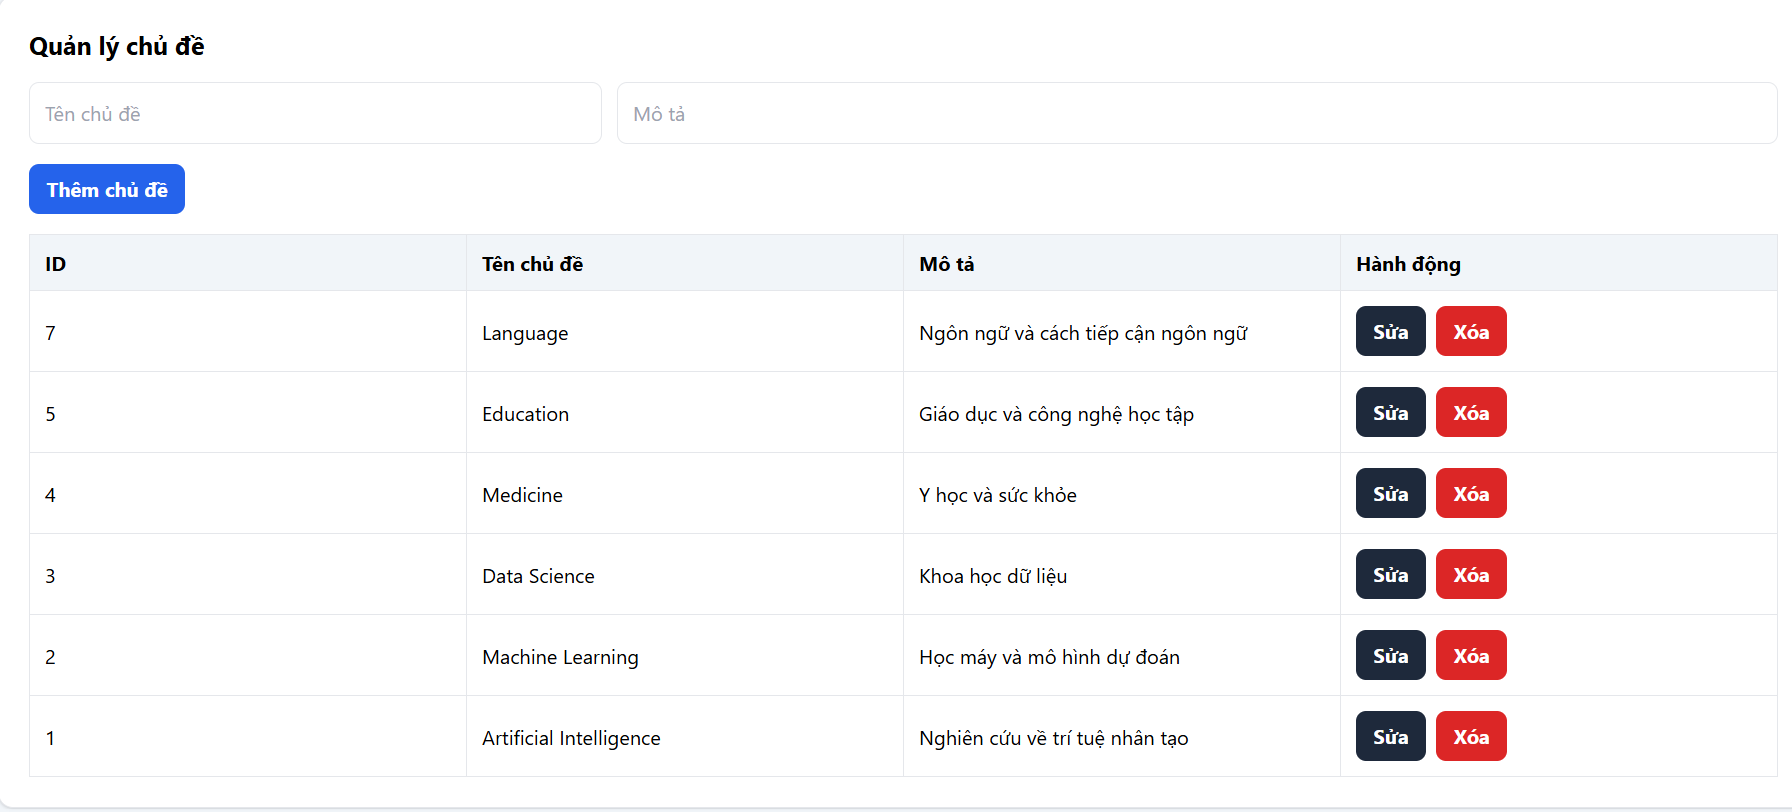
\includegraphics[width=6.5in,height=2.94514in]{media/media/image11.png}

\emph{Figure 3.11. Update the topic list after each action}

\subsection{3.5.3 API Source Management}\label{api-source-management}

Role: Admin

Function trigger: The admin opens the Admin page and selects Quản lý
nguồn API.

Function description:

- Purpose: Allow the admin to manage external API sources used by the
system.

- Data processing: Store and update API source information in the
database.

Function Details:

- Display the list of API sources.

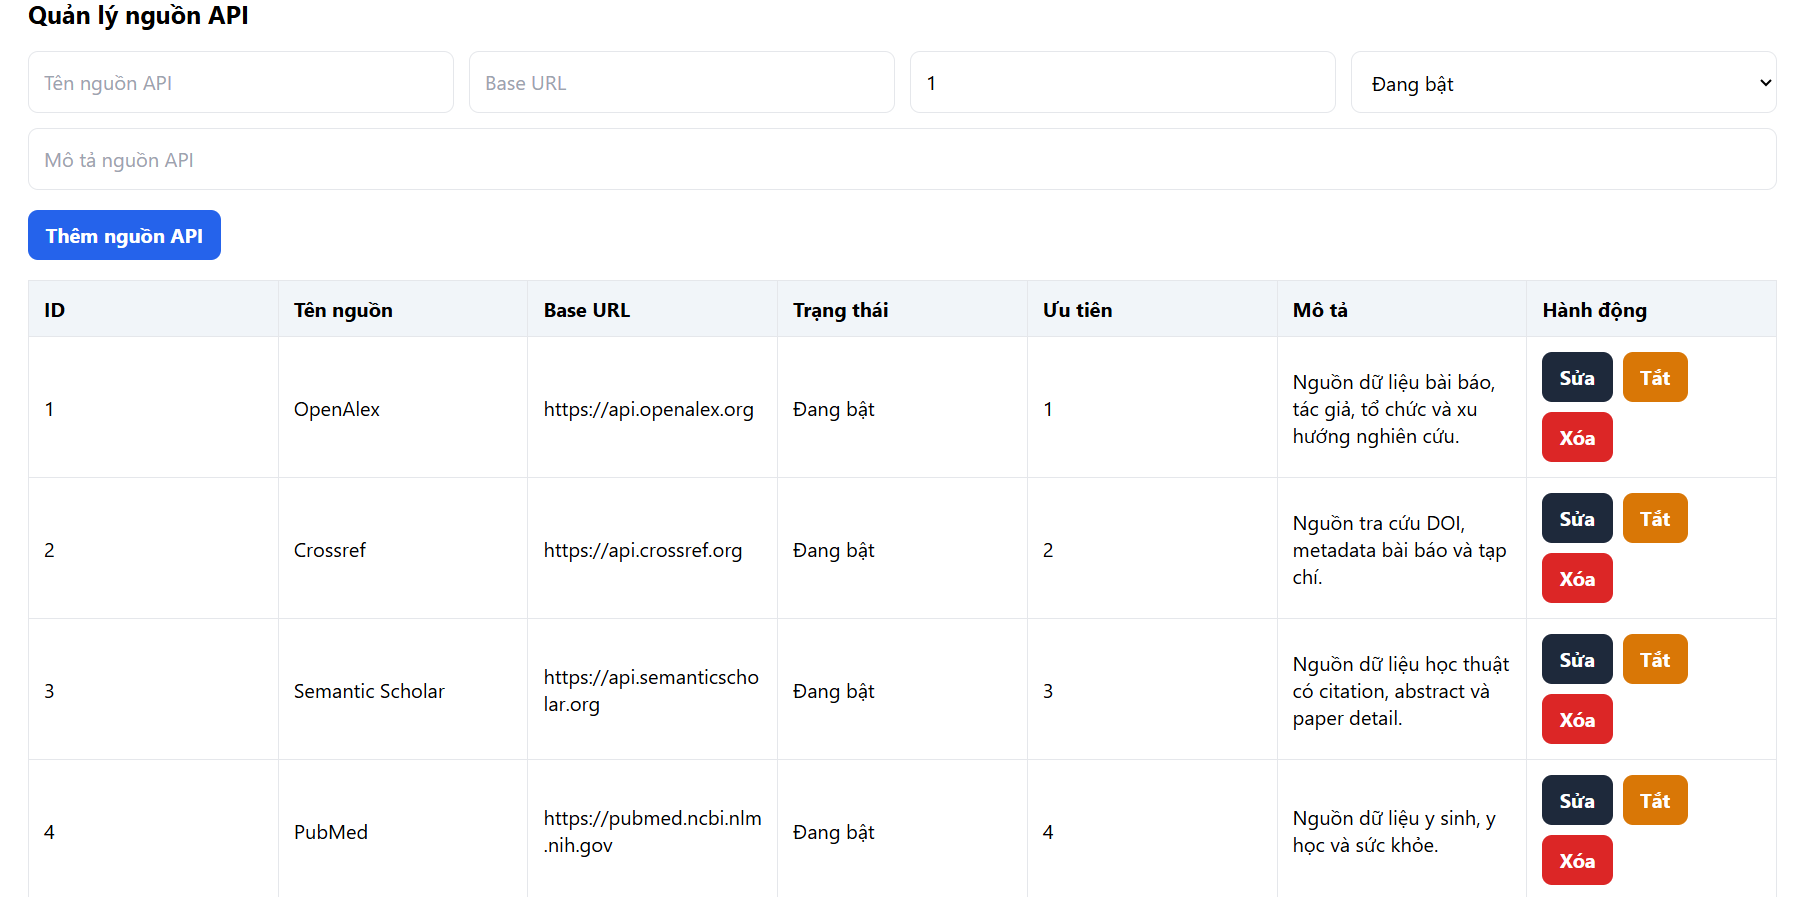
\includegraphics[width=6.5in,height=3.23542in]{media/media/image12.png}

\emph{Figure 3.12. API source management interface displaying the list
of external API sources}.

- Add a new API source.

- Edit API source name, base URL, status, priority, and description.

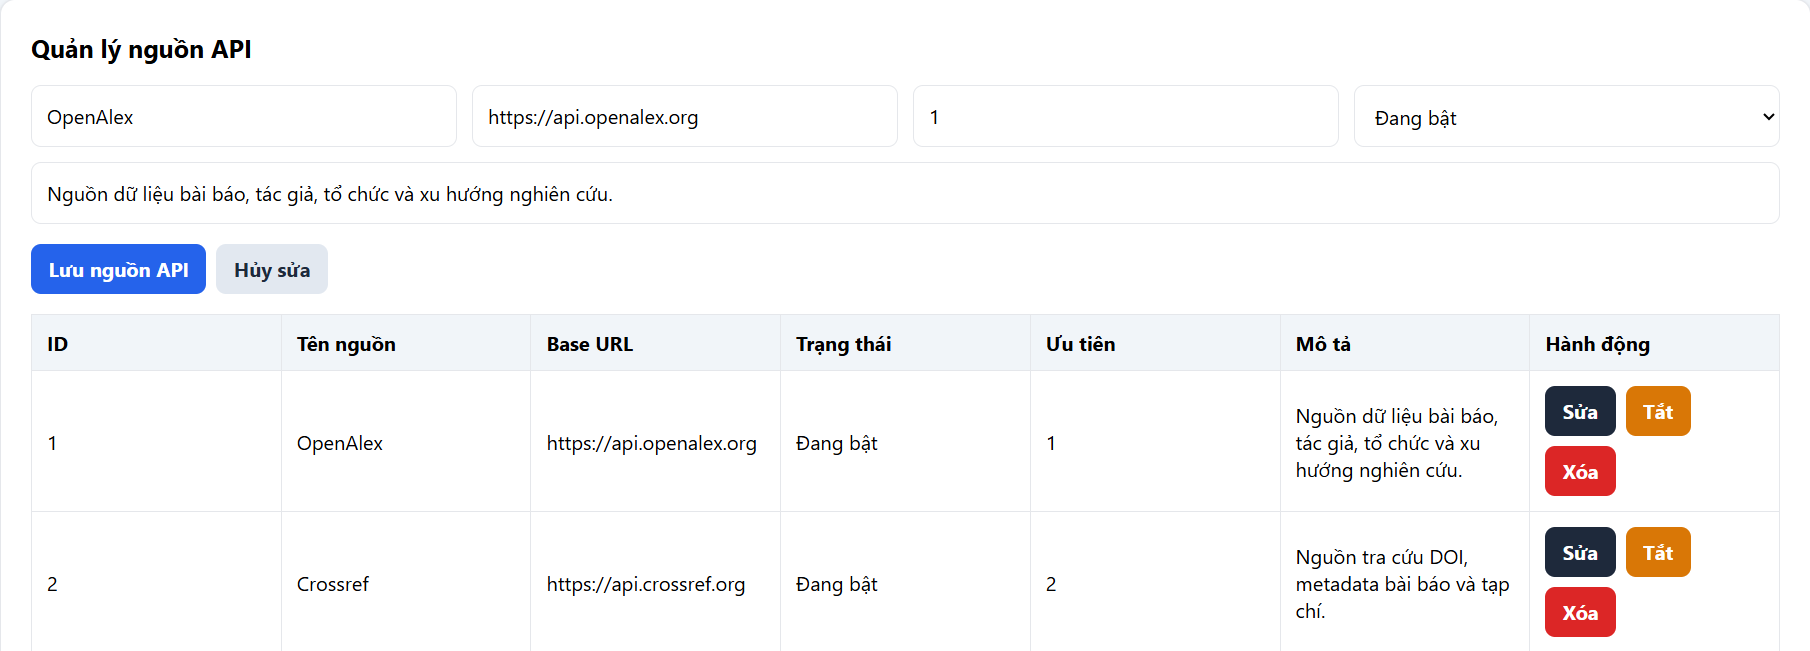
\includegraphics[width=6.5in,height=2.3375in]{media/media/image13.png}

\emph{Figure 3.13. Admin can edit API source information including name,
base URL, status, priority, and description.}

- Enable or disable an API source.

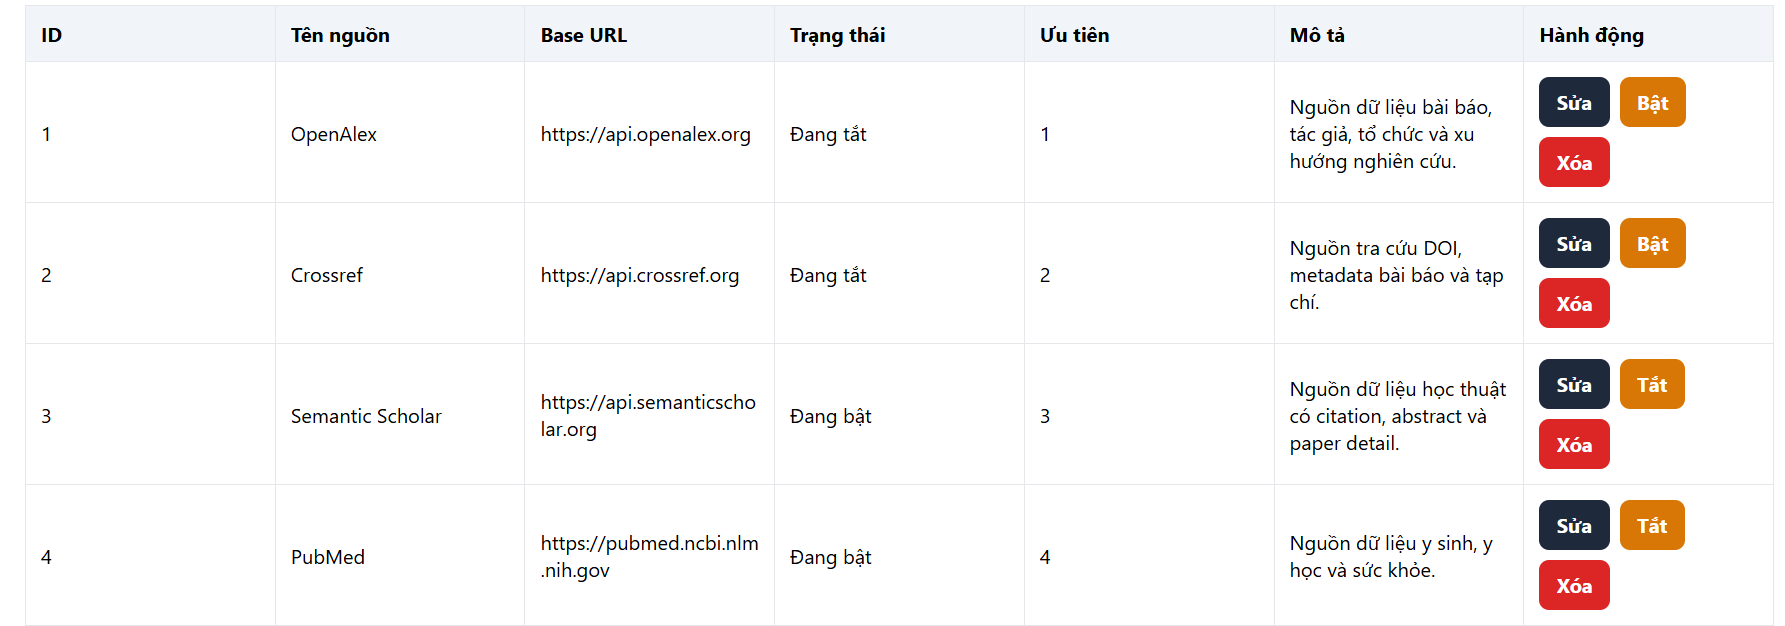
\includegraphics[width=6.5in,height=2.27917in]{media/media/image14.png}

\emph{Figure 3.14. Admin can enable or disable an API source.}

- Delete an API source.

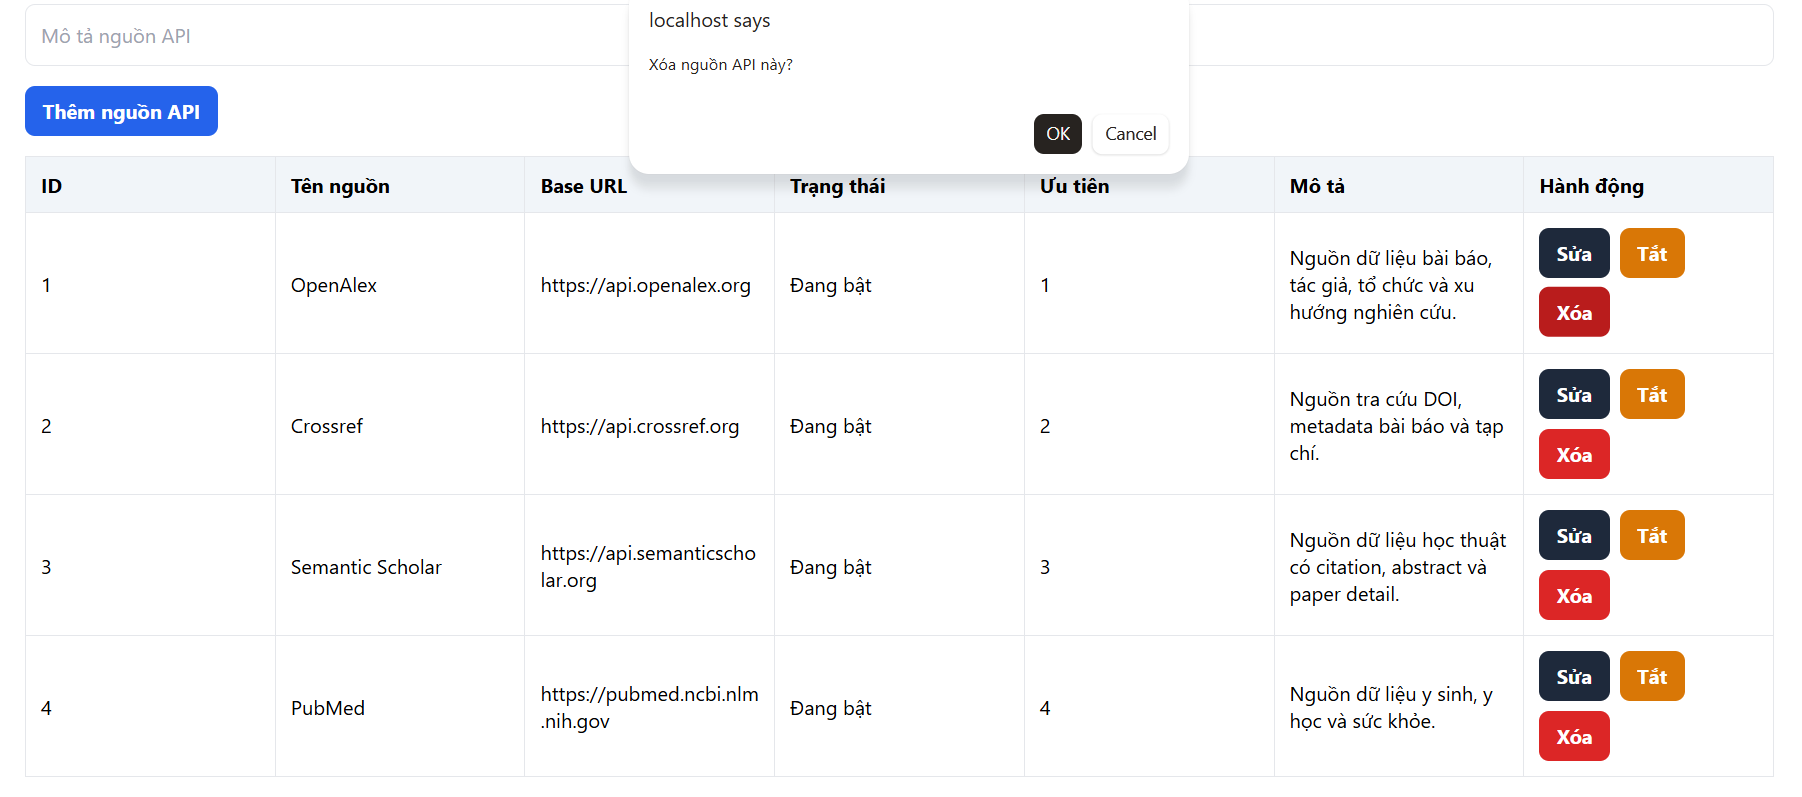
\includegraphics[width=6.5in,height=2.875in]{media/media/image15.png}

\emph{Figure 3.15. Admin can delete an external API source from the
system.}

\subsection{3.5.4 API Data
Synchronization}\label{api-data-synchronization}

Role: Admin

Function trigger: The admin clicks Đồng bộ hóa in the API
synchronization section.

Function description:

- Purpose: Synchronize data from external APIs into the system.

- Data processing: Fetch data from the selected API source, process the
returned data, update the research paper database, and save the
synchronization log.

Function Details:

- Select an API source.

- Enter a search keyword and the number of records to synchronize.

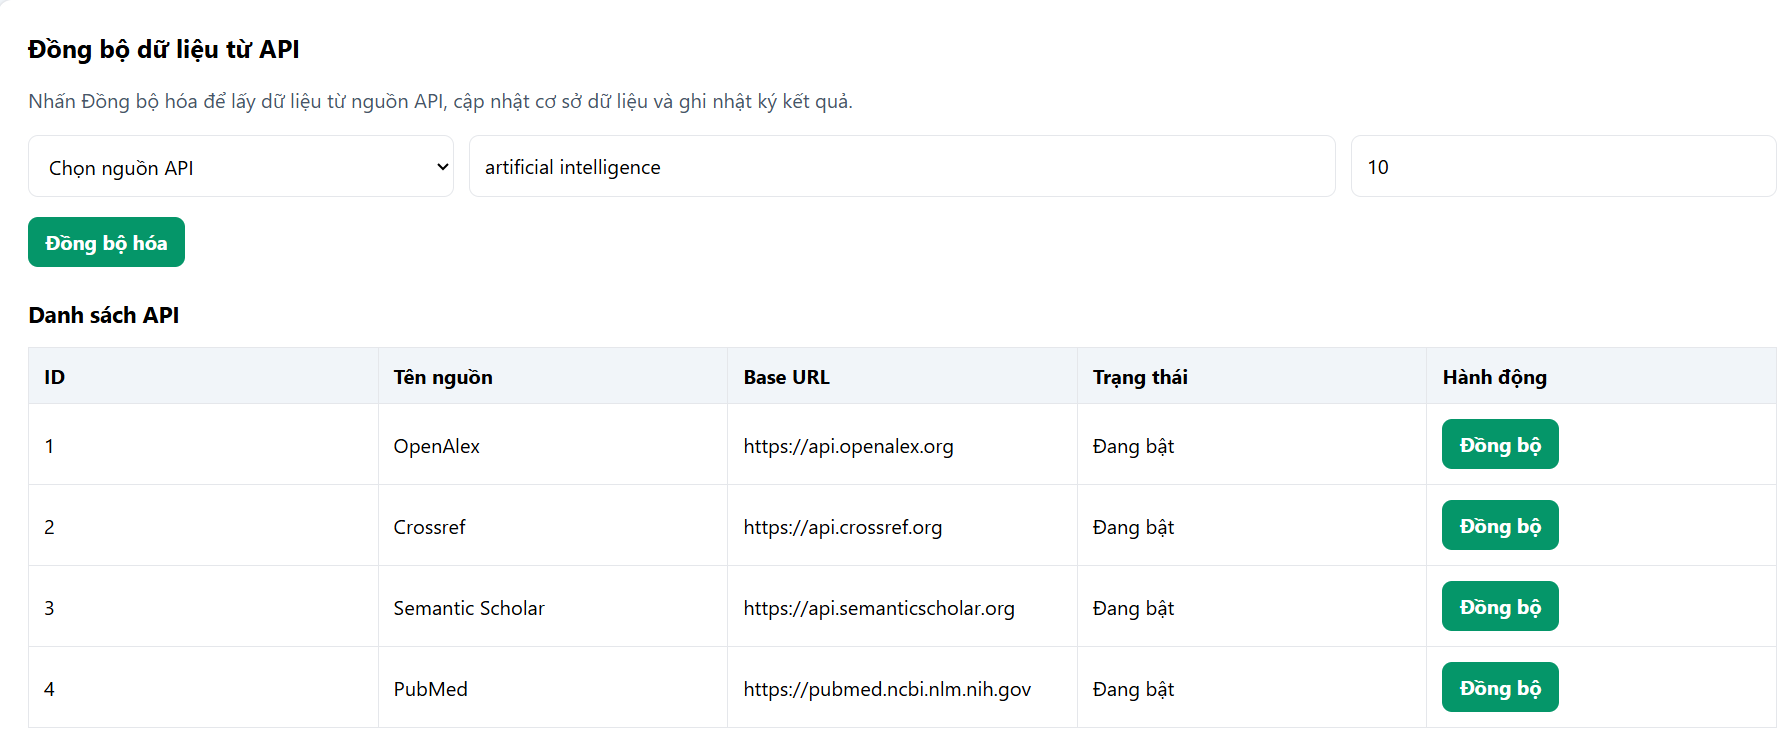
\includegraphics[width=6.5in,height=2.69097in]{media/media/image16.png}

\emph{Figure 3.16. API data synchronization form where admin selects an
API source, enters a keyword, and sets the number of records.}

- Click Đồng bộ hóa.

- The system fetches data from the external API.

- The system inserts new research papers or updates existing records.

- Display synchronization results including fetched, inserted, and
updated records.

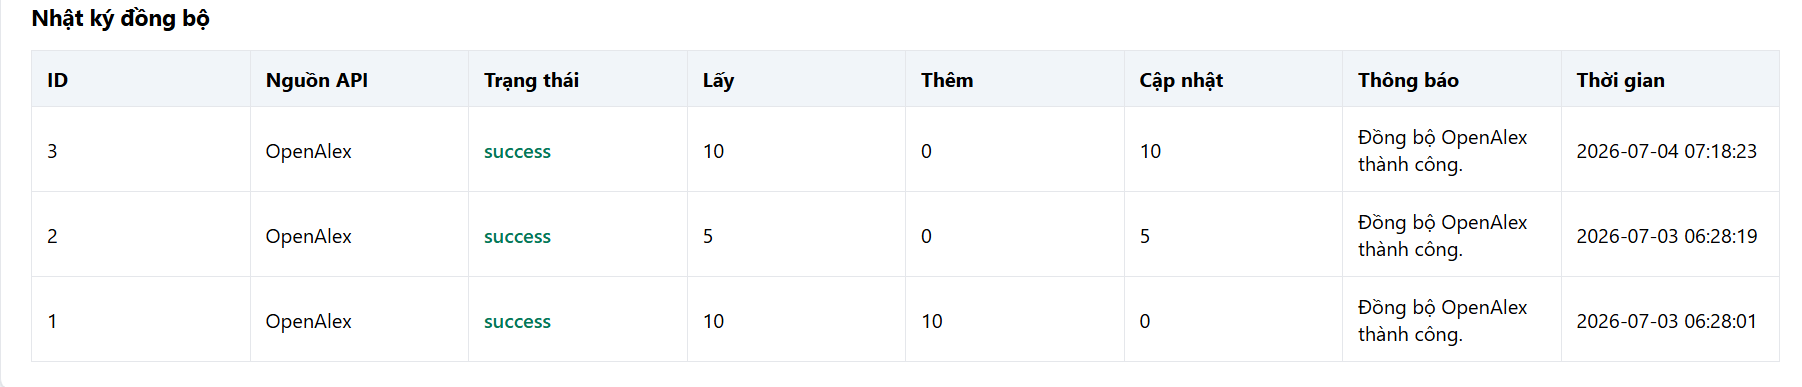
\includegraphics[width=6.5in,height=1.39583in]{media/media/image17.png}

\emph{Figure 3.17. The system displays synchronization results after
fetching data from the API}.

- Save the synchronization history in the synchronization log.

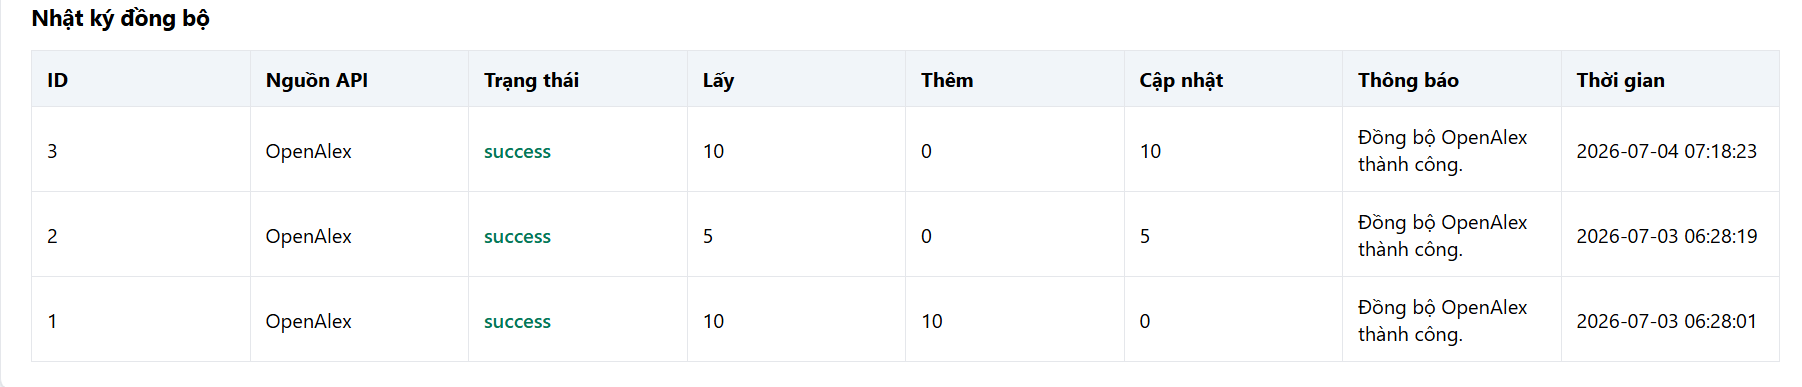
\includegraphics[width=6.5in,height=1.39583in]{media/media/image17.png}

\emph{Figure 3.18. The system displays synchronization results after
fetching data from the API.}

\subsection{3.5.5 Research Paper
Management}\label{research-paper-management}

Role: Admin

Function trigger: The admin opens the Admin page and selects Quản lý bài
báo.

Function description:

- Purpose: Allow the admin to manage research paper data.

- Data processing: Add, update, delete, and retrieve research paper
information from the database.

Function Details:

- Display the list of research papers.

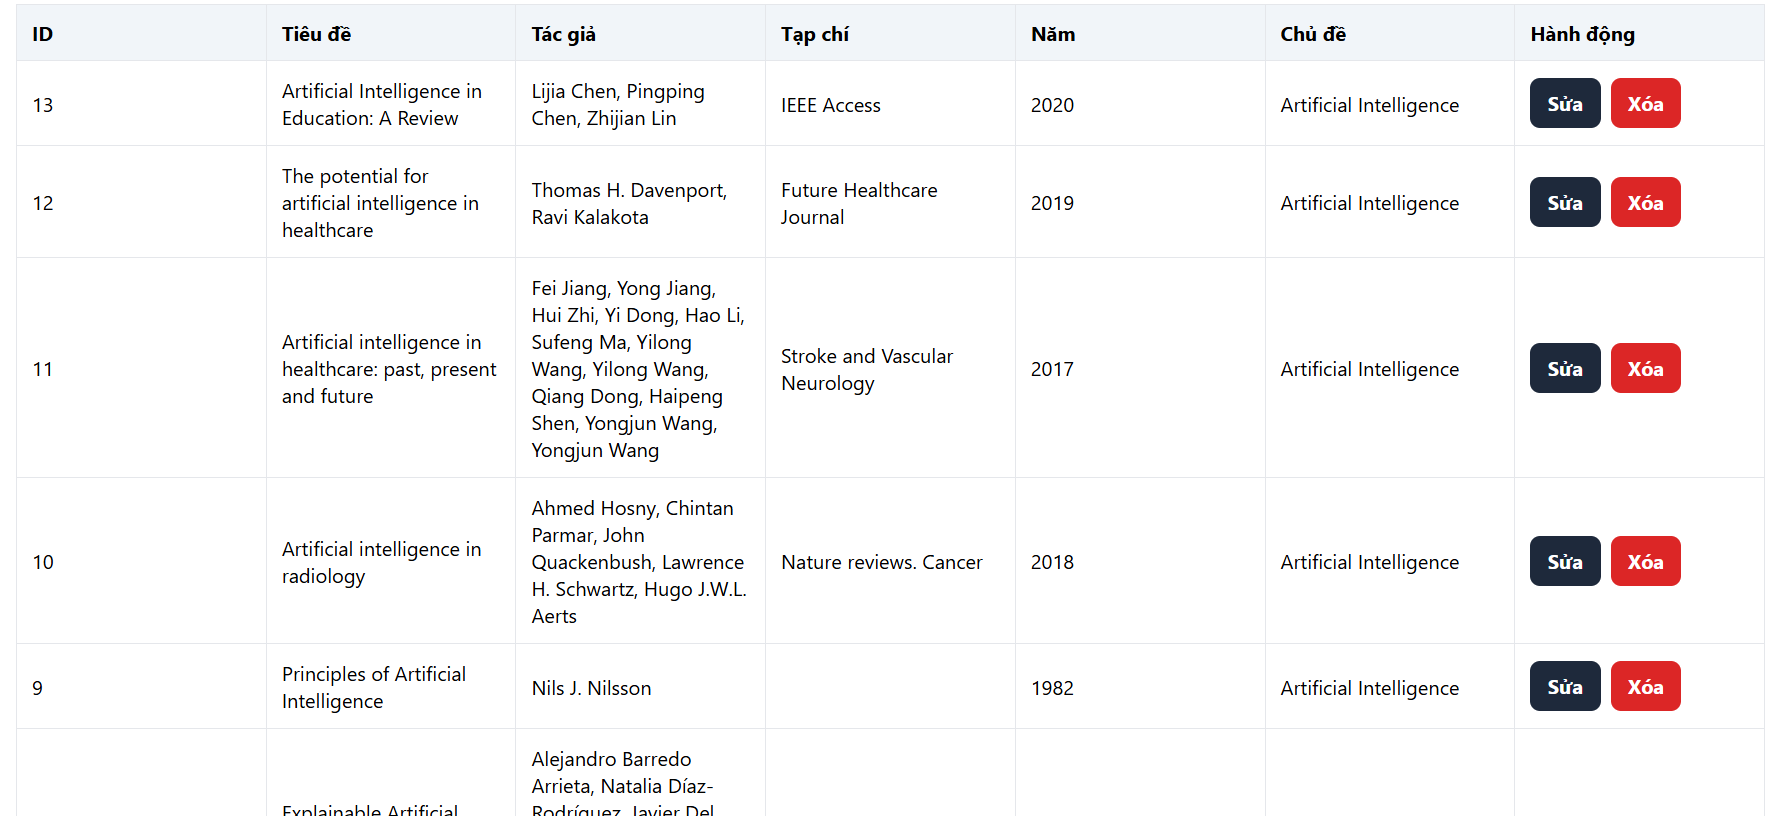
\includegraphics[width=6.5in,height=2.98472in]{media/media/image18.png}

\emph{Figure 3.19. Research paper management interface displaying the
list of research papers.}

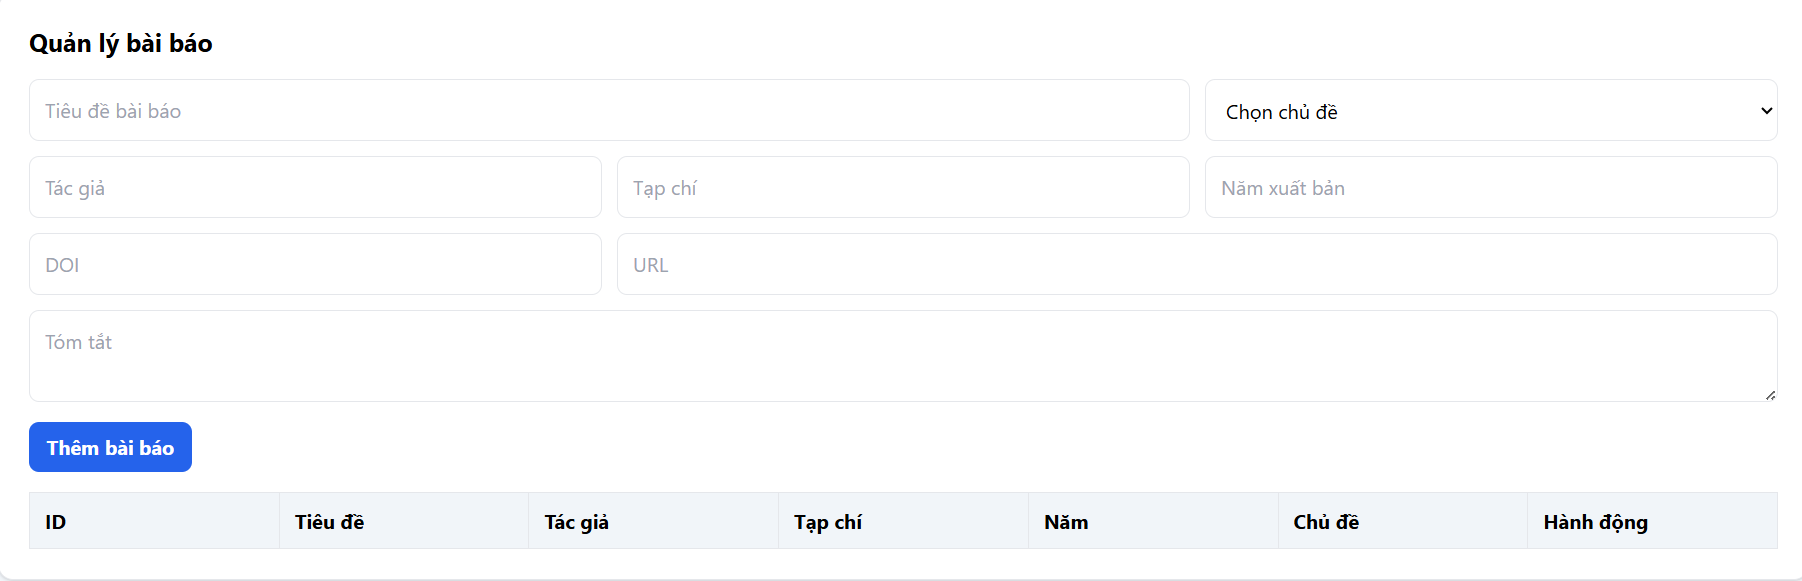
\includegraphics[width=6.5in,height=2.09583in]{media/media/image19.png}

\emph{Figure 3.20. Research paper management interface displaying the
list of research papers.}

- Add a new research paper.

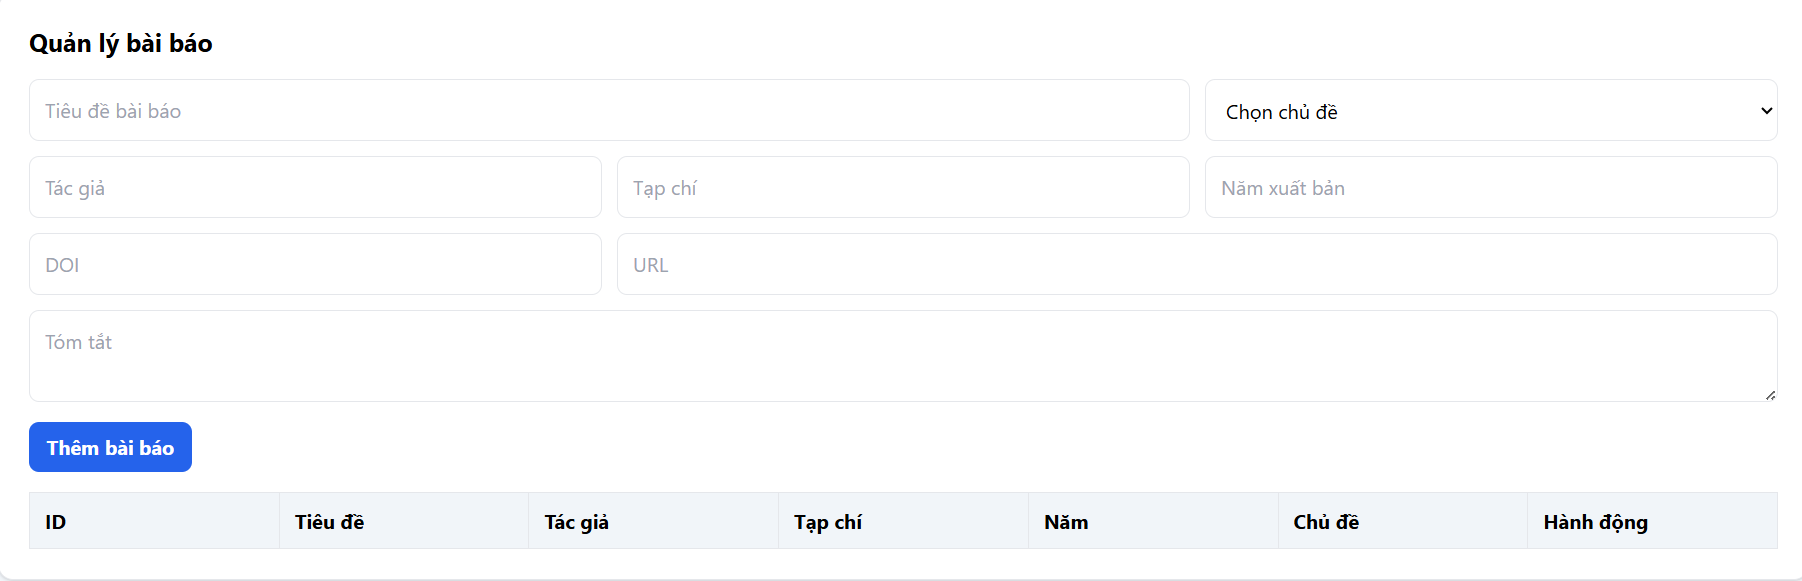
\includegraphics[width=6.5in,height=2.09583in]{media/media/image19.png}

\emph{Figure 3.21. Admin can add a new research paper by entering paper
information}.

- Edit title, authors, journal, publication year, DOI, URL, abstract,
and topic.

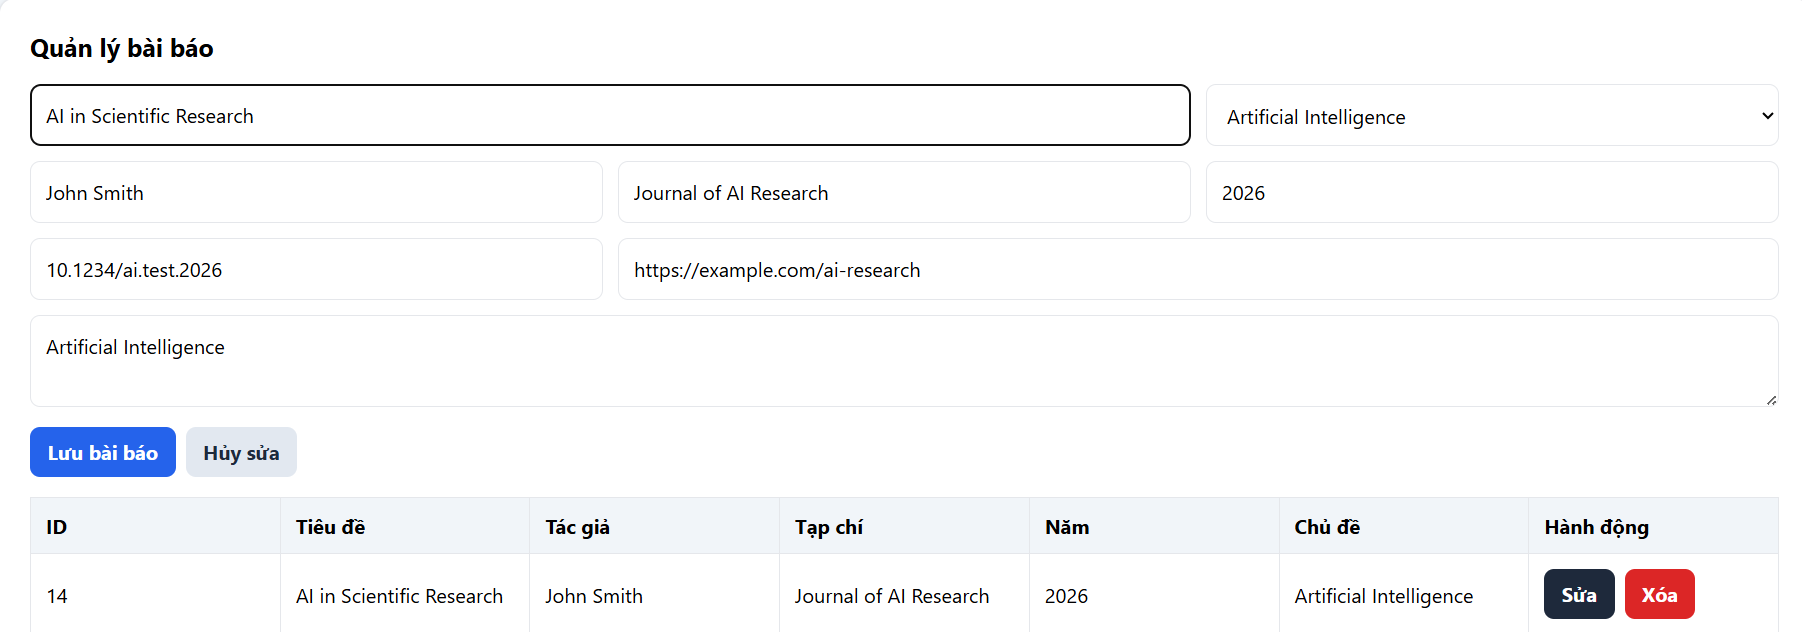
\includegraphics[width=6.5in,height=2.27986in]{media/media/image20.png}

\emph{Figure 3.22. Admin can edit research paper details including
title, authors, journal, year, DOI, URL, abstract, and topic.}

- Delete a research paper.

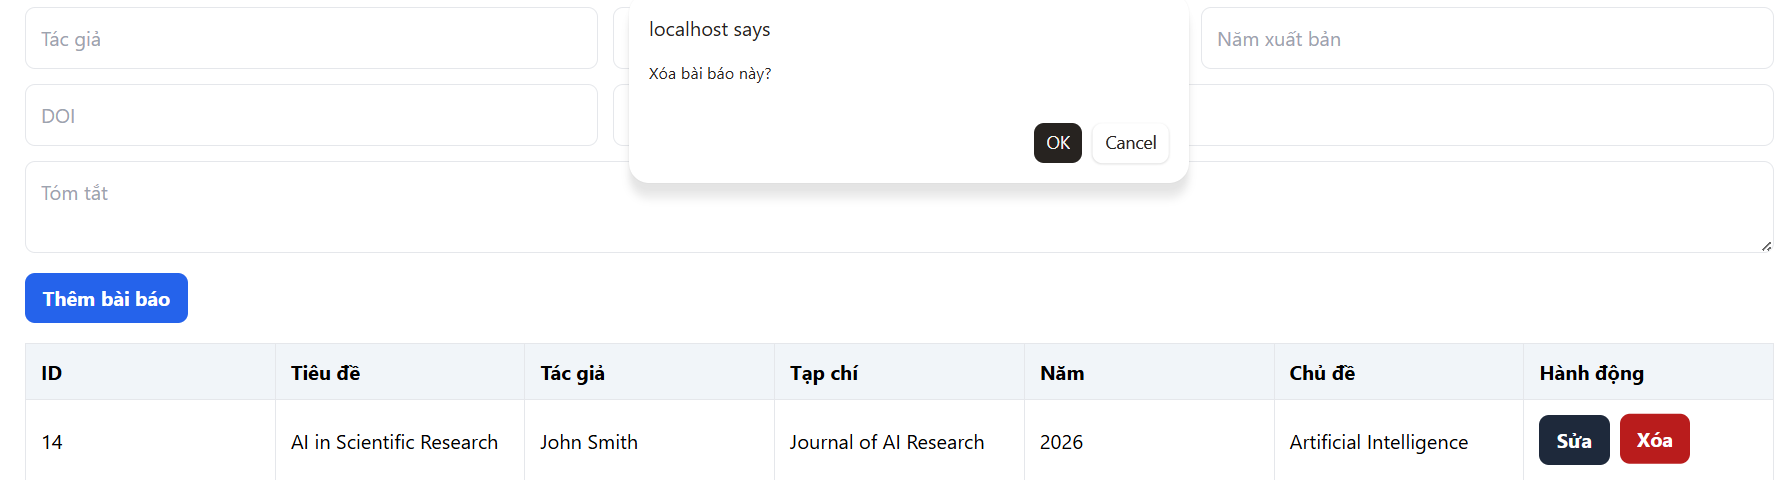
\includegraphics[width=6.5in,height=1.74792in]{media/media/image21.png}

\emph{Figure 3.23. Admin can delete a research paper from the system.}

- Update the paper list after each action.

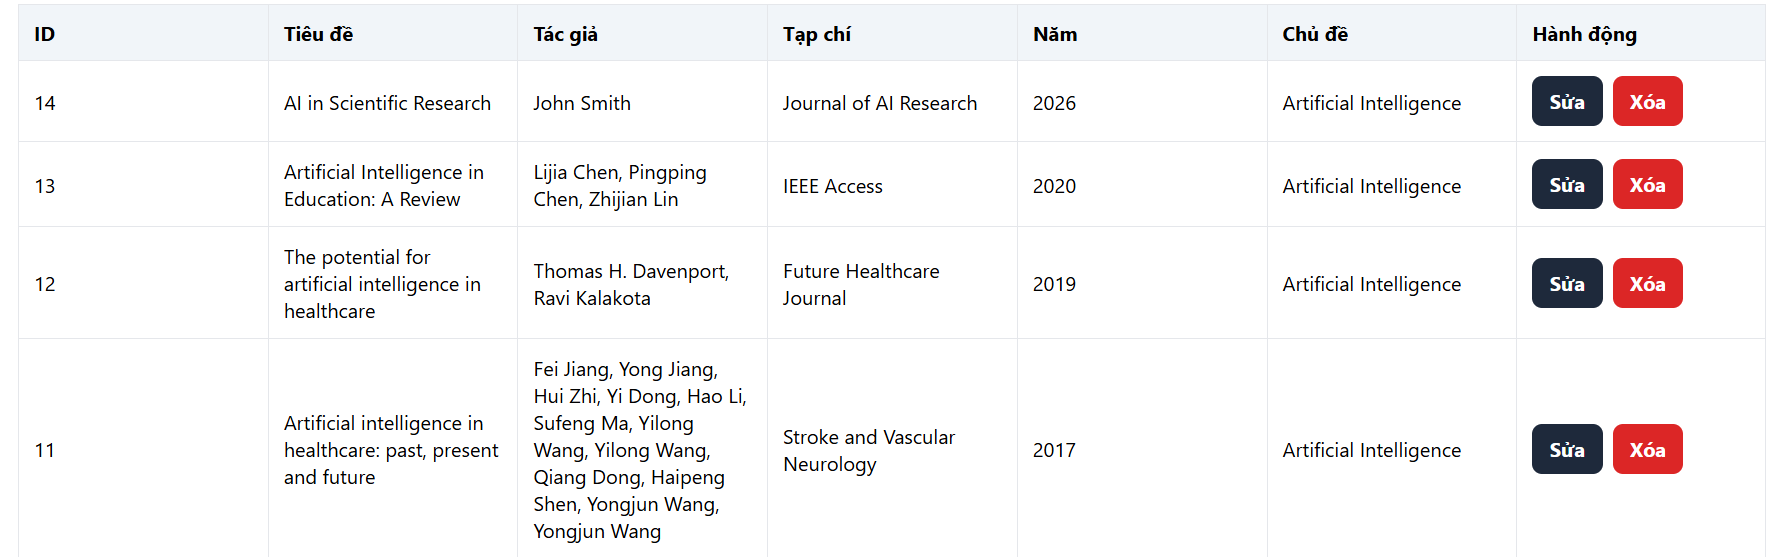
\includegraphics[width=6.5in,height=2.04861in]{media/media/image22.png}

\emph{Figure 3.24. The research paper list is updated after adding a new
paper.}

\subsection{3.5.6 Notification Management}\label{notification-management}

Role: Admin

Function trigger: The admin opens the Admin page and selects Quản lý
thông báo.

Function description:

- Purpose: Allow the admin to send and manage notifications for users.

- Data processing: Store notification data in the database and retrieve
notification history.

Function Details:

- Create a new notification with title, type, link, and content.

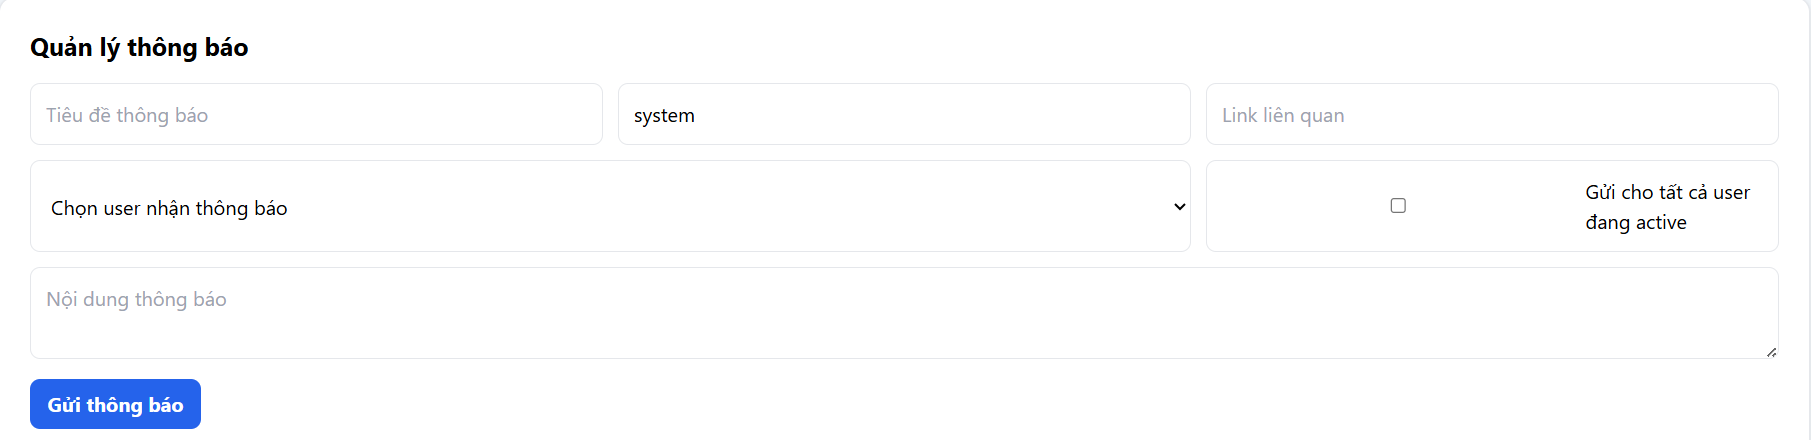
\includegraphics[width=6.5in,height=1.57917in]{media/media/image23.png}

\emph{Firgure 3.25. Notification Managment}

- Send a notification to one user or all active users.

- Display the list of sent notifications.

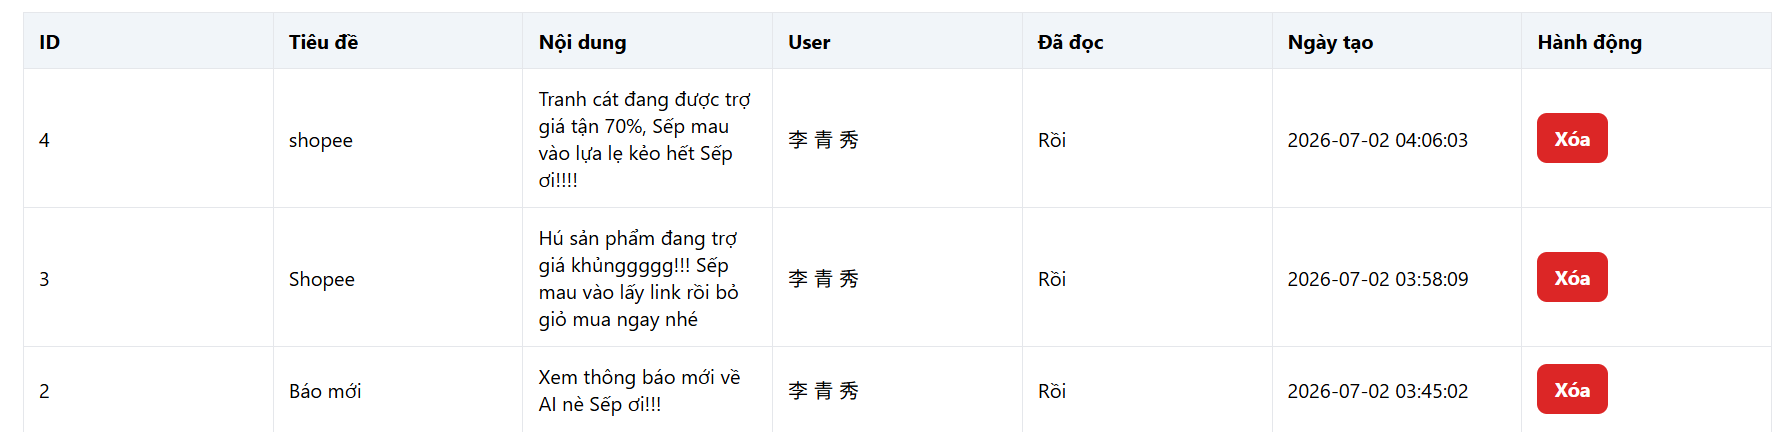
\includegraphics[width=6.5in,height=1.56667in]{media/media/image24.png}

\emph{Figure 3.26. Sent notifications are displayed in the notification
history list.}

- Delete a notification.

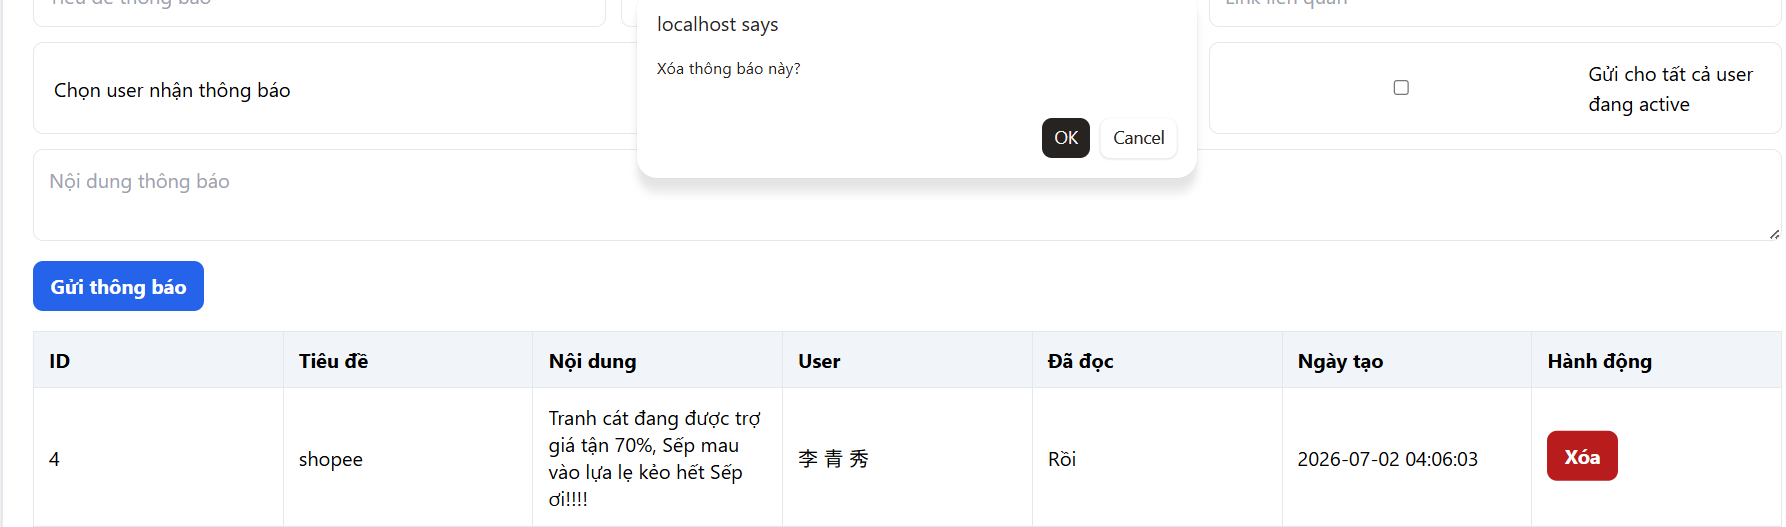
\includegraphics[width=6.5in,height=1.91806in]{media/media/image25.png}

\emph{Figure 3.27. Admin can delete a sent notification.}

- Users can view notifications on the notification page.

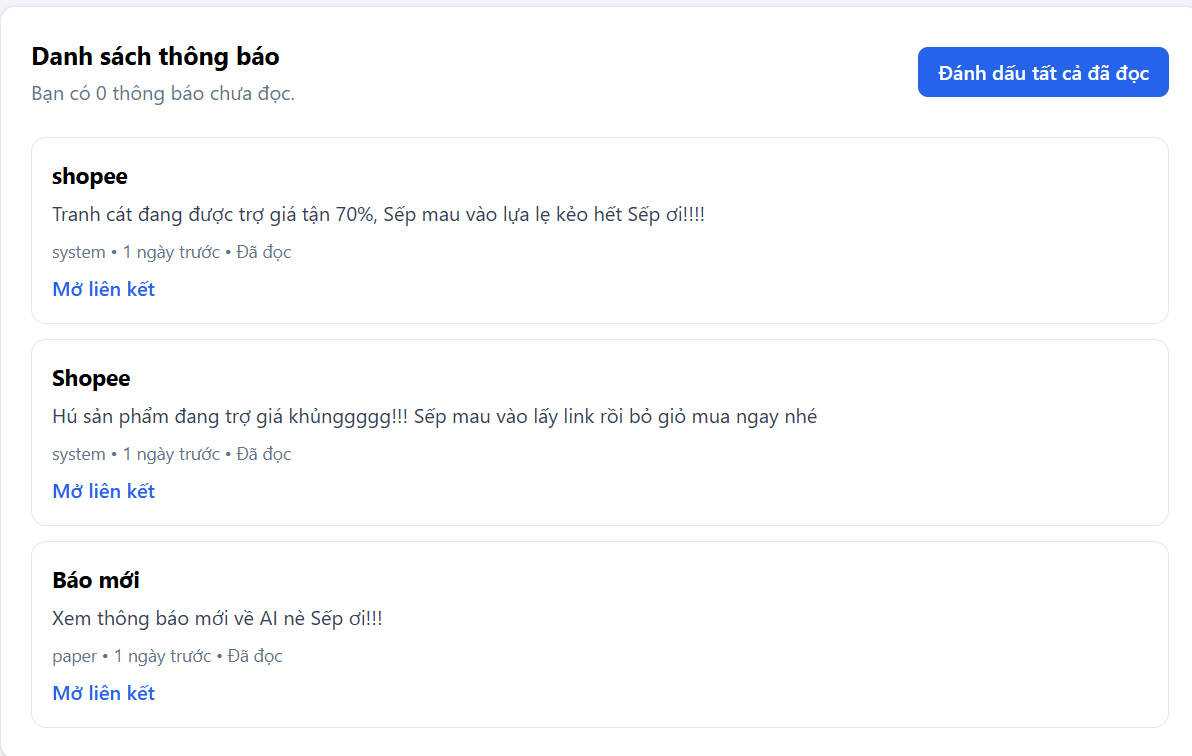
\includegraphics[width=6.5in,height=4.12222in]{media/media/image26.png}

\emph{Figure 3.28. User notification page showing notifications sent by
the admin.}

\end{document}
